\begin{tikzpicture}
\pgfdeclareplotmark{cross} {
\pgfpathmoveto{\pgfpoint{-0.3\pgfplotmarksize}{\pgfplotmarksize}}
\pgfpathlineto{\pgfpoint{+0.3\pgfplotmarksize}{\pgfplotmarksize}}
\pgfpathlineto{\pgfpoint{+0.3\pgfplotmarksize}{0.3\pgfplotmarksize}}
\pgfpathlineto{\pgfpoint{+1\pgfplotmarksize}{0.3\pgfplotmarksize}}
\pgfpathlineto{\pgfpoint{+1\pgfplotmarksize}{-0.3\pgfplotmarksize}}
\pgfpathlineto{\pgfpoint{+0.3\pgfplotmarksize}{-0.3\pgfplotmarksize}}
\pgfpathlineto{\pgfpoint{+0.3\pgfplotmarksize}{-1.\pgfplotmarksize}}
\pgfpathlineto{\pgfpoint{-0.3\pgfplotmarksize}{-1.\pgfplotmarksize}}
\pgfpathlineto{\pgfpoint{-0.3\pgfplotmarksize}{-0.3\pgfplotmarksize}}
\pgfpathlineto{\pgfpoint{-1.\pgfplotmarksize}{-0.3\pgfplotmarksize}}
\pgfpathlineto{\pgfpoint{-1.\pgfplotmarksize}{0.3\pgfplotmarksize}}
\pgfpathlineto{\pgfpoint{-0.3\pgfplotmarksize}{0.3\pgfplotmarksize}}
\pgfpathclose
\pgfusepathqstroke
}
\pgfdeclareplotmark{cross*} {
\pgfpathmoveto{\pgfpoint{-0.3\pgfplotmarksize}{\pgfplotmarksize}}
\pgfpathlineto{\pgfpoint{+0.3\pgfplotmarksize}{\pgfplotmarksize}}
\pgfpathlineto{\pgfpoint{+0.3\pgfplotmarksize}{0.3\pgfplotmarksize}}
\pgfpathlineto{\pgfpoint{+1\pgfplotmarksize}{0.3\pgfplotmarksize}}
\pgfpathlineto{\pgfpoint{+1\pgfplotmarksize}{-0.3\pgfplotmarksize}}
\pgfpathlineto{\pgfpoint{+0.3\pgfplotmarksize}{-0.3\pgfplotmarksize}}
\pgfpathlineto{\pgfpoint{+0.3\pgfplotmarksize}{-1.\pgfplotmarksize}}
\pgfpathlineto{\pgfpoint{-0.3\pgfplotmarksize}{-1.\pgfplotmarksize}}
\pgfpathlineto{\pgfpoint{-0.3\pgfplotmarksize}{-0.3\pgfplotmarksize}}
\pgfpathlineto{\pgfpoint{-1.\pgfplotmarksize}{-0.3\pgfplotmarksize}}
\pgfpathlineto{\pgfpoint{-1.\pgfplotmarksize}{0.3\pgfplotmarksize}}
\pgfpathlineto{\pgfpoint{-0.3\pgfplotmarksize}{0.3\pgfplotmarksize}}
\pgfpathclose
\pgfusepathqfillstroke
}
\pgfdeclareplotmark{newstar} {
\pgfpathmoveto{\pgfqpoint{0pt}{\pgfplotmarksize}}
\pgfpathlineto{\pgfqpointpolar{44}{0.5\pgfplotmarksize}}
\pgfpathlineto{\pgfqpointpolar{18}{\pgfplotmarksize}}
\pgfpathlineto{\pgfqpointpolar{-20}{0.5\pgfplotmarksize}}
\pgfpathlineto{\pgfqpointpolar{-54}{\pgfplotmarksize}}
\pgfpathlineto{\pgfqpointpolar{-90}{0.5\pgfplotmarksize}}
\pgfpathlineto{\pgfqpointpolar{234}{\pgfplotmarksize}}
\pgfpathlineto{\pgfqpointpolar{198}{0.5\pgfplotmarksize}}
\pgfpathlineto{\pgfqpointpolar{162}{\pgfplotmarksize}}
\pgfpathlineto{\pgfqpointpolar{134}{0.5\pgfplotmarksize}}
\pgfpathclose
\pgfusepathqstroke
}
\pgfdeclareplotmark{newstar*} {
\pgfpathmoveto{\pgfqpoint{0pt}{\pgfplotmarksize}}
\pgfpathlineto{\pgfqpointpolar{44}{0.5\pgfplotmarksize}}
\pgfpathlineto{\pgfqpointpolar{18}{\pgfplotmarksize}}
\pgfpathlineto{\pgfqpointpolar{-20}{0.5\pgfplotmarksize}}
\pgfpathlineto{\pgfqpointpolar{-54}{\pgfplotmarksize}}
\pgfpathlineto{\pgfqpointpolar{-90}{0.5\pgfplotmarksize}}
\pgfpathlineto{\pgfqpointpolar{234}{\pgfplotmarksize}}
\pgfpathlineto{\pgfqpointpolar{198}{0.5\pgfplotmarksize}}
\pgfpathlineto{\pgfqpointpolar{162}{\pgfplotmarksize}}
\pgfpathlineto{\pgfqpointpolar{134}{0.5\pgfplotmarksize}}
\pgfpathclose
\pgfusepathqfillstroke
}
\definecolor{c}{rgb}{1,1,1};
\draw [color=c, fill=c] (0,0) rectangle (20,14.3108);
\draw [color=c, fill=c] (3.2,2.28972) rectangle (19,13.5952);
\definecolor{c}{rgb}{0,0,0};
\draw [c,line width=0.9] (3.2,2.28972) -- (3.2,13.5952) -- (19,13.5952) -- (19,2.28972) -- (3.2,2.28972);
\definecolor{c}{rgb}{0.1802,0.7178,0.6425};
\draw [color=c, fill=c] (3.2,2.28972) rectangle (6.53333,4.40951);
\definecolor{c}{rgb}{0.453559,0.742331,0.504766};
\draw [color=c, fill=c] (6.53333,2.28972) rectangle (9.86667,4.40951);
\definecolor{c}{rgb}{0.956881,0.774519,0.230291};
\draw [color=c, fill=c] (9.86667,2.28972) rectangle (12.3333,4.40951);
\draw [color=c, fill=c] (13.3333,2.28972) rectangle (16.5333,4.40951);
\definecolor{c}{rgb}{0.9842,0.903169,0.111953};
\draw [color=c, fill=c] (16.5333,2.28972) rectangle (19,4.40951);
\definecolor{c}{rgb}{0.1802,0.7178,0.6425};
\draw [color=c, fill=c] (3.2,4.40951) rectangle (6.53333,5.8227);
\definecolor{c}{rgb}{0.116419,0.686966,0.702991};
\draw [color=c, fill=c] (6.53333,4.40951) rectangle (9.86667,5.8227);
\definecolor{c}{rgb}{0.322347,0.730556,0.570878};
\draw [color=c, fill=c] (9.86667,4.40951) rectangle (12.3333,5.8227);
\definecolor{c}{rgb}{0.956881,0.774519,0.230291};
\draw [color=c, fill=c] (13.3333,4.40951) rectangle (16.5333,5.8227);
\definecolor{c}{rgb}{0.977,0.977044,0.0583656};
\draw [color=c, fill=c] (16.5333,4.40951) rectangle (19,5.8227);
\definecolor{c}{rgb}{0.0526375,0.656131,0.763481};
\draw [color=c, fill=c] (3.2,5.8227) rectangle (6.53333,7.94248);
\draw [color=c, fill=c] (6.53333,5.8227) rectangle (9.86667,7.94248);
\definecolor{c}{rgb}{0.116419,0.686966,0.702991};
\draw [color=c, fill=c] (9.86667,5.8227) rectangle (12.3333,7.94248);
\definecolor{c}{rgb}{0.701397,0.739462,0.397147};
\draw [color=c, fill=c] (13.3333,5.8227) rectangle (16.5333,7.94248);
\definecolor{c}{rgb}{0.956881,0.774519,0.230291};
\draw [color=c, fill=c] (16.5333,5.8227) rectangle (19,7.94248);
\definecolor{c}{rgb}{0.0526375,0.656131,0.763481};
\draw [color=c, fill=c] (3.2,7.94248) rectangle (6.53333,13.5952);
\definecolor{c}{rgb}{0.033475,0.616063,0.800231};
\draw [color=c, fill=c] (6.53333,7.94248) rectangle (9.86667,13.5952);
\definecolor{c}{rgb}{0.0526375,0.656131,0.763481};
\draw [color=c, fill=c] (9.86667,7.94248) rectangle (12.3333,13.5952);
\definecolor{c}{rgb}{0.701397,0.739462,0.397147};
\draw [color=c, fill=c] (13.3333,7.94248) rectangle (16.5333,13.5952);
\definecolor{c}{rgb}{0.8186,0.7328,0.3499};
\draw [color=c, fill=c] (16.5333,7.94248) rectangle (19,13.5952);
\definecolor{c}{rgb}{0,0,0};
\draw (4.86667,3.34962) node[scale=1.61424, color=c, rotate=1]{$\genfrac{}{}{0pt}{}{0.0127}{\pm 0.0002}$};
\draw (8.2,3.34962) node[scale=1.61424, color=c, rotate=1]{$\genfrac{}{}{0pt}{}{0.0151}{\pm 0.0000}$};
\draw (11.1,3.34962) node[scale=1.61424, color=c, rotate=1]{$\genfrac{}{}{0pt}{}{0.0213}{\pm 0.0001}$};
\draw (14.9333,3.34962) node[scale=1.61424, color=c, rotate=1]{$\genfrac{}{}{0pt}{}{0.0216}{\pm 0.0002}$};
\draw (17.7667,3.34962) node[scale=1.61424, color=c, rotate=1]{$\genfrac{}{}{0pt}{}{0.0246}{\pm 0.0000}$};
\draw (4.86667,5.1161) node[scale=1.61424, color=c, rotate=1]{$\genfrac{}{}{0pt}{}{0.0120}{\pm 0.0001}$};
\draw (8.2,5.1161) node[scale=1.61424, color=c, rotate=1]{$\genfrac{}{}{0pt}{}{0.0118}{\pm 0.0002}$};
\draw (11.1,5.1161) node[scale=1.61424, color=c, rotate=1]{$\genfrac{}{}{0pt}{}{0.0142}{\pm 0.0002}$};
\draw (14.9333,5.1161) node[scale=1.61424, color=c, rotate=1]{$\genfrac{}{}{0pt}{}{0.0213}{\pm 0.0002}$};
\draw (17.7667,5.1161) node[scale=1.61424, color=c, rotate=1]{$\genfrac{}{}{0pt}{}{0.0265}{\pm 0.0002}$};
\draw (4.86667,6.88259) node[scale=1.61424, color=c, rotate=1]{$\genfrac{}{}{0pt}{}{0.0094}{\pm 0.0001}$};
\draw (8.2,6.88259) node[scale=1.61424, color=c, rotate=1]{$\genfrac{}{}{0pt}{}{0.0100}{\pm 0.0001}$};
\draw (11.1,6.88259) node[scale=1.61424, color=c, rotate=1]{$\genfrac{}{}{0pt}{}{0.0111}{\pm 0.0001}$};
\draw (14.9333,6.88259) node[scale=1.61424, color=c, rotate=1]{$\genfrac{}{}{0pt}{}{0.0183}{\pm 0.0002}$};
\draw (17.7667,6.88259) node[scale=1.61424, color=c, rotate=1]{$\genfrac{}{}{0pt}{}{0.0214}{\pm 0.0002}$};
\draw (4.86667,10.7689) node[scale=1.61424, color=c, rotate=1]{$\genfrac{}{}{0pt}{}{0.0093}{\pm 0.0002}$};
\draw (8.2,10.7689) node[scale=1.61424, color=c, rotate=1]{$\genfrac{}{}{0pt}{}{0.0091}{\pm 0.0005}$};
\draw (11.1,10.7689) node[scale=1.61424, color=c, rotate=1]{$\genfrac{}{}{0pt}{}{0.0094}{\pm 0.0003}$};
\draw (14.9333,10.7689) node[scale=1.61424, color=c, rotate=1]{$\genfrac{}{}{0pt}{}{0.0178}{\pm 0.0004}$};
\draw (17.7667,10.7689) node[scale=1.61424, color=c, rotate=1]{$\genfrac{}{}{0pt}{}{0.0195}{\pm 0.0006}$};
\draw [c,line width=0.9] (3.2,2.28972) -- (19,2.28972);
\draw [anchor=north] (4.86667,2.12014) node[scale=1.0576, color=c, rotate=0]{[0.0 - 0.5]};
\draw [anchor=north] (8.2,2.12014) node[scale=1.0576, color=c, rotate=0]{[0.5 - 1.0]};
\draw [anchor=north] (11.1,2.12014) node[scale=1.0576, color=c, rotate=0]{[1.0 - 1.37]};
% \draw [anchor=north] (12.8333,2.12014) node[scale=1.0576, color=c, rotate=0]{[1.37 - 1.52]};
\draw [anchor=north] (14.9333,2.12014) node[scale=1.0576, color=c, rotate=0]{[1.52 - 2.0]};
\draw [anchor=north] (17.7667,2.12014) node[scale=1.0576, color=c, rotate=0]{[2.0 - 2.37]};
\draw [c,line width=0.9] (3.2,2.62889) -- (3.2,2.28972);
\draw [c,line width=0.9] (6.53333,2.62889) -- (6.53333,2.28972);
\draw [c,line width=0.9] (9.86667,2.62889) -- (9.86667,2.28972);
\draw [c,line width=0.9] (13.2,2.62889) -- (13.2,2.28972);
\draw [c,line width=0.9] (16.5333,2.62889) -- (16.5333,2.28972);
\draw [c,line width=0.9] (16.5333,2.62889) -- (16.5333,2.28972);
\draw [anchor= east] (19,0.686917) node[scale=1.61424, color=c, rotate=0]{$|\eta|_{  e}^{probe}$};
\draw [c,line width=0.9] (3.2,13.5952) -- (19,13.5952);
\draw [c,line width=0.9] (3.2,13.2561) -- (3.2,13.5952);
\draw [c,line width=0.9] (6.53333,13.2561) -- (6.53333,13.5952);
\draw [c,line width=0.9] (9.86667,13.2561) -- (9.86667,13.5952);
\draw [c,line width=0.9] (13.2,13.2561) -- (13.2,13.5952);
\draw [c,line width=0.9] (16.5333,13.2561) -- (16.5333,13.5952);
\draw [c,line width=0.9] (16.5333,13.2561) -- (16.5333,13.5952);
\draw [c,line width=0.9] (3.2,2.28972) -- (3.2,13.5952);
\draw [anchor= east] (2.963,3.34962) node[scale=1.0576, color=c, rotate=0]{[20 - 35] };
\draw [anchor= east] (2.963,5.1161) node[scale=1.0576, color=c, rotate=0]{[35 - 45] };
\draw [anchor= east] (2.963,6.88259) node[scale=1.0576, color=c, rotate=0]{[45 - 60] };
\draw [anchor= east] (2.963,8.6) node[scale=1.0576, color=c, rotate=0]{[60 - 100]};
\draw [c,line width=0.9] (3.674,2.28972) -- (3.2,2.28972);
\draw [c,line width=0.9] (3.674,5.1161) -- (3.2,5.1161);
\draw [c,line width=0.9] (3.674,7.94248) -- (3.2,7.94248);
\draw [c,line width=0.9] (3.674,10.7689) -- (3.2,10.7689);
\draw [c,line width=0.9] (3.674,13.5952) -- (3.2,13.5952);
\draw [anchor= east] (0.96,13.5952) node[scale=1.61424, color=c, rotate=90]{$p_{T,  e}^{probe}  [GeV]$};
\draw [c,line width=0.9] (19,2.28972) -- (19,13.5952);
\draw [c,line width=0.9] (18.526,2.28972) -- (19,2.28972);
\draw [c,line width=0.9] (18.526,5.1161) -- (19,5.1161);
\draw [c,line width=0.9] (18.526,7.94248) -- (19,7.94248);
\draw [c,line width=0.9] (18.526,10.7689) -- (19,10.7689);
\draw [c,line width=0.9] (18.526,13.5952) -- (19,13.5952);
\definecolor{c}{rgb}{0.150523,0.241303,0.660565};
\draw [color=c, fill=c] (19.1,2.28972) rectangle (19.99,2.855);
\definecolor{c}{rgb}{0.0880387,0.322448,0.802768};
\draw [color=c, fill=c] (19.1,2.855) rectangle (19.99,3.42028);
\definecolor{c}{rgb}{0.0633125,0.391444,0.861859};
\draw [color=c, fill=c] (19.1,3.42028) rectangle (19.99,3.98555);
\definecolor{c}{rgb}{0.0703625,0.445519,0.850647};
\draw [color=c, fill=c] (19.1,3.98555) rectangle (19.99,4.55083);
\definecolor{c}{rgb}{0.078,0.5041,0.8385};
\draw [color=c, fill=c] (19.1,4.55083) rectangle (19.99,5.1161);
\definecolor{c}{rgb}{0.0557375,0.560081,0.819366};
\draw [color=c, fill=c] (19.1,5.1161) rectangle (19.99,5.68138);
\definecolor{c}{rgb}{0.033475,0.616063,0.800231};
\draw [color=c, fill=c] (19.1,5.68138) rectangle (19.99,6.24665);
\definecolor{c}{rgb}{0.0526375,0.656131,0.763481};
\draw [color=c, fill=c] (19.1,6.24665) rectangle (19.99,6.81193);
\definecolor{c}{rgb}{0.116419,0.686966,0.702991};
\draw [color=c, fill=c] (19.1,6.81193) rectangle (19.99,7.37721);
\definecolor{c}{rgb}{0.1802,0.7178,0.6425};
\draw [color=c, fill=c] (19.1,7.37721) rectangle (19.99,7.94248);
\definecolor{c}{rgb}{0.322347,0.730556,0.570878};
\draw [color=c, fill=c] (19.1,7.94248) rectangle (19.99,8.50776);
\definecolor{c}{rgb}{0.453559,0.742331,0.504766};
\draw [color=c, fill=c] (19.1,8.50776) rectangle (19.99,9.07303);
\definecolor{c}{rgb}{0.584194,0.746125,0.444394};
\draw [color=c, fill=c] (19.1,9.07303) rectangle (19.99,9.63831);
\definecolor{c}{rgb}{0.701397,0.739462,0.397147};
\draw [color=c, fill=c] (19.1,9.63831) rectangle (19.99,10.2036);
\definecolor{c}{rgb}{0.8186,0.7328,0.3499};
\draw [color=c, fill=c] (19.1,10.2036) rectangle (19.99,10.7689);
\definecolor{c}{rgb}{0.884975,0.752825,0.292488};
\draw [color=c, fill=c] (19.1,10.7689) rectangle (19.99,11.3341);
\definecolor{c}{rgb}{0.956881,0.774519,0.230291};
\draw [color=c, fill=c] (19.1,11.3341) rectangle (19.99,11.8994);
\definecolor{c}{rgb}{0.992,0.823138,0.170006};
\draw [color=c, fill=c] (19.1,11.8994) rectangle (19.99,12.4647);
\definecolor{c}{rgb}{0.9842,0.903169,0.111953};
\draw [color=c, fill=c] (19.1,12.4647) rectangle (19.99,13.03);
\definecolor{c}{rgb}{0.977,0.977044,0.0583656};
\draw [color=c, fill=c] (19.1,13.03) rectangle (19.99,13.5952);
\definecolor{c}{rgb}{0,0,0};
\draw [c,line width=0.9] (19.99,2.28972) -- (19.99,13.5952);
\draw [c,line width=0.9] (19.516,2.28972) -- (19.99,2.28972);
\draw [c,line width=0.9] (19.516,4.42485) -- (19.99,4.42485);
\draw [c,line width=0.9] (19.516,6.55997) -- (19.99,6.55997);
\draw [c,line width=0.9] (19.516,8.6951) -- (19.99,8.6951);
\draw [c,line width=0.9] (19.516,10.8302) -- (19.99,10.8302);
\draw [c,line width=0.9] (19.516,12.9653) -- (19.99,12.9653);
\draw [c,line width=0.9] (19.516,12.9653) -- (19.99,12.9653);
\draw [anchor= west] (20.09,2.28972) node[scale=1.61424, color=c, rotate=0]{0};
\draw [anchor= west] (20.09,4.42485) node[scale=1.61424, color=c, rotate=0]{0.005};
\draw [anchor= west] (20.09,6.55997) node[scale=1.61424, color=c, rotate=0]{0.01};
\draw [anchor= west] (20.09,8.6951) node[scale=1.61424, color=c, rotate=0]{0.015};
\draw [anchor= west] (20.09,10.8302) node[scale=1.61424, color=c, rotate=0]{0.02};
\draw [anchor= west] (20.09,12.9653) node[scale=1.61424, color=c, rotate=0]{0.025};
\end{tikzpicture}
